%Version 3 October 2023
% See section 11 of the User Manual for version history
%
%%%%%%%%%%%%%%%%%%%%%%%%%%%%%%%%%%%%%%%%%%%%%%%%%%%%%%%%%%%%%%%%%%%%%%
%%                                                                 %%
%% Please do not use \input{...} to include other tex files.       %%
%% Submit your LaTeX manuscript as one .tex document.              %%
%%                                                                 %%
%% All additional figures and files should be attached             %%
%% separately and not embedded in the \TeX\ document itself.       %%
%%                                                                 %%
%%%%%%%%%%%%%%%%%%%%%%%%%%%%%%%%%%%%%%%%%%%%%%%%%%%%%%%%%%%%%%%%%%%%%

%%\documentclass[referee,sn-basic]{sn-jnl}% referee option is meant for double line spacing

%%=======================================================%%
%% to print line numbers in the margin use lineno option %%
%%=======================================================%%

%%\documentclass[lineno,sn-basic]{sn-jnl}% Basic Springer Nature Reference Style/Chemistry Reference Style

%%======================================================%%
%% to compile with pdflatex/xelatex use pdflatex option %%
%%======================================================%%

%%\documentclass[pdflatex,sn-basic]{sn-jnl}% Basic Springer Nature Reference Style/Chemistry Reference Style


%%Note: the following reference styles support Namedate and Numbered referencing. By default the style follows the most common style. To switch between the options you can add or remove �Numbered� in the optional parenthesis.
%%The option is available for: sn-basic.bst, sn-vancouver.bst, sn-chicago.bst%

%%\documentclass[sn-nature]{sn-jnl}% Style for submissions to Nature Portfolio journals
%%\documentclass[sn-basic]{sn-jnl}% Basic Springer Nature Reference Style/Chemistry Reference Style
\documentclass[sn-mathphys-num]{sn-jnl}% Math and Physical Sciences Numbered Reference Style
%%\documentclass[sn-mathphys-ay]{sn-jnl}% Math and Physical Sciences Author Year Reference Style
%%\documentclass[sn-aps]{sn-jnl}% American Physical Society (APS) Reference Style
%%\documentclass[sn-vancouver,Numbered]{sn-jnl}% Vancouver Reference Style
%%\documentclass[sn-apa]{sn-jnl}% APA Reference Style
%%\documentclass[sn-chicago]{sn-jnl}% Chicago-based Humanities Reference Style

%%%% Standard Packages
%%<additional latex packages if required can be included here>
%% MY PACKAGE
\usepackage[detect-all=true]{siunitx}
\sisetup{
    round-mode = places,
    round-precision = 2
}

\usepackage{pifont}% http://ctan.org/pkg/pifont
\newcommand{\cmark}{\ding{51}}%
\newcommand{\xmark}{\ding{55}}%
\usepackage[acronym, automake, style=index, shortcuts]{glossaries-extra}
\setabbreviationstyle[acronym]{long-short}

% define new commands
\makeglossaries
\newacronym{blat}{BLAT}{BLAST-like alignment tool}
\newacronym{blast}{BLAST}{Basic Local Alignment Search Tool}
\newacronym{cli}{CLI}{Command-Line Interface}
\newacronym{api}{API}{Application Programming Interface}
\newacronym{ide}{IDE}{Integrated Development Environment}
\newacronym{gil}{GIL}{Global Interpreter Lock}
\newacronym{ci}{CI}{Continuous Integration}
\newacronym{cd}{CD}{Continuous Development}
\newacronym{ucsc}{UCSC}{UCSC Genome Browser}
\newacronym{hsp}{HSP}{High-Scoring Pair}
\newglossaryentry{pxblat}{name=PxBLAT, description={pxblat}}
%% MY PACKAGE

\usepackage{graphicx}%
\usepackage{multirow}%
\usepackage{amsmath,amssymb,amsfonts}%
\usepackage{amsthm}%
\usepackage{mathrsfs}%
\usepackage[title]{appendix}%
\usepackage{xcolor}%
\usepackage{textcomp}%
\usepackage{manyfoot}%
\usepackage{booktabs}%
\usepackage{algorithm}%
\usepackage{algorithmicx}%
\usepackage{algpseudocode}%
\usepackage{listings}%
\usepackage{minted}


%%%%%=============================================================================%%%%
%%%%  Remarks: This template is provided to aid authors with the preparation
%%%%  of original research articles intended for submission to journals published
%%%%  by Springer Nature. The guidance has been prepared in partnership with
%%%%  production teams to conform to Springer Nature technical requirements.
%%%%  Editorial and presentation requirements differ among journal portfolios and
%%%%  research disciplines. You may find sections in this template are irrelevant
%%%%  to your work and are empowered to omit any such section if allowed by the
%%%%  journal you intend to submit to. The submission guidelines and policies
%%%%  of the journal take precedence. A detailed User Manual is available in the
%%%%  template package for technical guidance.
%%%%%=============================================================================%%%%

%% as per the requirement new theorem styles can be included as shown below
\theoremstyle{thmstyleone}%
\newtheorem{theorem}{Theorem}%  meant for continuous numbers
%%\newtheorem{theorem}{Theorem}[section]% meant for sectionwise numbers
%% optional argument [theorem] produces theorem numbering sequence instead of independent numbers for Proposition
\newtheorem{proposition}[theorem]{Proposition}%
%%\newtheorem{proposition}{Proposition}% to get separate numbers for theorem and proposition etc.

\theoremstyle{thmstyletwo}%
\newtheorem{example}{Example}%
\newtheorem{remark}{Remark}%

\theoremstyle{thmstylethree}%
\newtheorem{definition}{Definition}%

\raggedbottom
\unnumbered% uncomment this for unnumbered level heads

\begin{document}

\title[Article Title]{PxBLAT: An efficient python binding library for BLAT}

%%=============================================================%%
%% GivenName	-> \fnm{Joergen W.}
%% Particle	-> \spfx{van der} -> surname prefix
%% FamilyName	-> \sur{Ploeg}
%% Suffix	-> \sfx{IV}
%% \author*[1,2]{\fnm{Joergen W.} \spfx{van der} \sur{Ploeg}
%%  \sfx{IV}}\email{iauthor@gmail.com}
%%=============================================================%%

\author[1]{\fnm{Yangyang} \sur{Li}}\email{yangyang.li@northwestern.edu}

\author*[1]{\fnm{Rendong} \sur{Yang}}\email{rendong.yang@northwestern.edu}
%\equalcont{These authors contributed equally to this work.}

%\author[1,2]{\fnm{Third} \sur{Author}}\email{iiiauthor@gmail.com}
%\equalcont{These authors contributed equally to this work.}

\affil[1]{\orgdiv{Department of Urology}, \orgname{Northwestern University Feinberg School of Medicine}, \orgaddress{\street{303 E Superior St}, \city{Chicago}, \postcode{60611}, \state{IL}, \country{USA}}}

%
%\affil[2]{\orgdiv{Department}, \orgname{Organization}, \orgaddress{\street{Street}, \city{City}, \postcode{10587}, \state{State}, \country{Country}}}
%
%\affil[3]{\orgdiv{Department}, \orgname{Organization}, \orgaddress{\street{Street}, \city{City}, \postcode{610101}, \state{State}, \country{Country}}}

%%==================================%%
%% Sample for unstructured abstract %%
%%==================================%%

%\abstract{The abstract serves both as a general introduction to the topic and as a brief, non-technical summary of the main results and their implications. Authors are advised to check the author instructions for the journal they are submitting to for word limits and if structural elements like subheadings, citations, or equations are permitted.}

%%================================%%
%% Sample for structured abstract %%
%%================================%%
\abstract{\textbf{Background:} With the surge in genomic data driven by advancements in sequencing technologies, the demand for efficient bioinformatics tools for sequence analysis has become paramount.
    \gls{blat}, a sequence alignment tool, faces limitations in performance efficiency and integration with modern programming environments, particularly Python.
    This study introduces \gls{pxblat}, a Python-based framework designed to enhance the capabilities of \gls{blat}, focusing on usability, computational efficiency, and seamless integration within the Python ecosystem.
	
	\textbf{Results:} \gls{pxblat} demonstrates significant improvements over \gls{blat} in execution speed and data handling, as evidenced by comprehensive benchmarks conducted across various sample groups ranging from 50 to 600 samples.
    These experiments highlight a notable speedup, achieving a reduction in execution time compared to \gls{blat}.
    The framework also introduces user-friendly features such as improved server management, data conversion utilities, and shell completion, enhancing the overall user experience.
    Additionally, the provision of extensive documentation and comprehensive testing supports community engagement and facilitates the adoption of \gls{pxblat}.
	
	\textbf{Conclusions:} \gls{pxblat} stands out as a robust alternative to \gls{blat}, offering enhancements in performance and user interaction.
    Its development underscores the potential for modern programming languages to improve bioinformatics tools, aligning with the needs of contemporary genomic research.
    By providing a more efficient, user-friendly tool, \gls{pxblat} has the potential to impact genomic data analysis workflows, supporting faster and more accurate sequence analysis in a Python environment.
}

\keywords{Software Libraries, Sequence Analysis, BLAT}

%%\pacs[JEL Classification]{D8, H51}
%%\pacs[MSC Classification]{35A01, 65L10, 65L12, 65L20, 65L70}

\maketitle

\section{Background}\label{sec1}

The rise of Python as a preferred programming language within bioinformatics is widely acknowledged as a result of its user-friendly nature, extensive libraries, and unparalleled versatility~\cite{perkel2015programming}.
A variety of libraries have been crafted to augment Python's interface, thereby amplifying the adaptability and compatibility of bioinformatics tools~\cite{putri2022analysing, cock2009biopython}.
For instance, Biopython~\cite{cock2009biopython}, a preeminent bioinformatics library, furnishes interfaces to tools like \gls{blast}~\cite{altschul1990basic} and Clustal~\cite{higgins1988clustal}.
\gls{blat}, a prominent tool in bioinformatics, is renowned for its speed in genome sequence alignments and serves as a more efficient alternative to \gls{blast} for aligning DNA sequences with the reference genome~\cite{kent2002blat,grant2011comparative,borozan2013evaluation}.
Furthermore, the unprecedented growth in genome sequencing technologies has significantly increased the availability of genomic data, emphasizing the need for advanced tools in both research and clinical contexts~\cite{mardis2008next,marx2023method}.

Despite its popularity and effectiveness, \gls{blat}'s integration is fraught with difficulties, primarily due to its C-based implementation and reliance on \glspl{cli}, hindering seamless integration into Python projects~\cite{wang2019pblat}.
Also, executing extensive queries with the \gls{blat} suite leads to inefficiencies when operations are isolated and not executed in batches.
Typically, \gls{blat}'s task allocation is sporadic, intermixed with other tasks.
Users generally face a choice: either employ standalone \gls{blat} or integrate \emph{gfServer} with \emph{gfClient}~\cite{altschul1990basic}.
\gls{blat}'s standard operational model involves initiating \emph{gfServer}, conducting the sequence query through \emph{gfClient}, and subsequently terminating the server after each query.
This method becomes highly inefficient for ungrouped, numerous queries as it necessitates the repeated initialization and shutdown of \emph{gfServer}, introducing significant overhead~\cite{kent2002blat}.
An optimized approach would entail initiating \emph{gfServer} a single time and leveraging \emph{gfClient} to execute multiple queries.
However, the command-line-only access to \emph{gfServer} and \emph{gfClient} complicates this process.
This limitation necessitates the management of system calls (like \emph{subprocess} or \emph{os.system}), the handling of intermediate temporary files, and dealing with format conversion, all of which cumulatively degrade performance.

\gls{pxblat} is proposed as a solution that allows for the programmatic use of \gls{blat}, ensuring its smooth integration into new algorithms or analytical pipelines within the Python ecosystem.
It acts as a conduit, merging the high-performance capabilities of \gls{blat} with Python's versatility while ensuring data reproducibility.
The primary goal of \gls{pxblat} is to bridge the gap in the current landscape by providing a Python binding library tailored specifically for \gls{blat}, addressing both the efficiency bottlenecks and the ergonomic challenges of its integration.

\section{Implementation}\label{sec:implementation}

The design of \gls{pxblat} is anchored in the principles of readability and simplicity, fostering an intuitive user interface that minimizes the learning curve for users.
In our quest to streamline complexity and amplify both usability and performance, we meticulously extracted the core implementation of \gls{blat} from the broader \gls{ucsc} codebase, significantly reducing dependency overhead.

We preserved the integrity of the original C codebase while reimplementing key \gls{blat} \(\left(\mathtt{V}37.1\right)\) utilities such as \emph{faTwoBit}, \emph{gfServer}, and \emph{gfClient} in C\texttt{++}.
This strategic choice not only modernizes the code but also enhances maintainability and scalability.
The integration of the revamped C\texttt{++} code with \gls{pxblat} was achieved using Pybind11~\cite{pybind11}, a lightweight, seamless method for interfacing C\texttt{++} and Python.

This approach ensures a direct and efficient interaction with \gls{blat}'s functions, upholding the original performance benchmarks and reliability of \gls{blat}.
Simultaneously, it extends the framework's functionality, aligning it with modern computational standards and making it a robust tool in the bioinformatics toolkit (Table~\ref{tab:apicmp}).

\begin{table}[!ht]
	\centering
	\caption{{\bf Overview of features of \gls{pxblat} compared with \gls{blat}.}}\label{tab:apicmp}
	\begin{tabular}{@{}lll@{}}
		\toprule
		Feature          & \gls{pxblat} & \gls{blat} \\ \midrule
		start server     & \cmark{}     & \cmark{}   \\
		stop  server     & \cmark{}     & \cmark{}   \\
		query server     & \cmark{}     & \cmark{}   \\
		wait server      & \cmark{}     & \xmark{}   \\
		fasta to bit     & \cmark{}     & \xmark{}   \\
		bit to fasta     & \cmark{}     & \xmark{}   \\
		port retry       & \cmark{}     & \xmark{}   \\
		shell completion & \cmark{}     & \xmark{}   \\
		\bottomrule
	\end{tabular}
	\footnotetext{
		This table presents a comprehensive comparison between the features offered by \gls{pxblat} and \gls{blat}.
		Features are denoted with a \cmark{} to signify availability and an \xmark{} to indicate absence.
		Notably, \gls{pxblat} showcases significant enhancements, particularly in server management (e.g., wait server), data conversion (e.g., fasta to bit, bit to fasta), and enriched user interaction (e.g., shell completion).
		These advancements firmly establish \gls{pxblat} as a superior and more versatile alternative to the conventional \gls{blat} tool.
	}
\end{table}

\gls{pxblat} features \gls{cli} utilities crafted through its \glspl{api}, boasting shell completion for various systems to augment its versatility (Table~\ref{tab:apicmp}).
Recognizing the diverse technological landscape, we provide the library in wheel format compatible with multiple platforms, including Linux x86-64, macOS x86-64, and macOS arm64.
This ensures a seamless installation process, free from the complexities of C library dependencies, making it straightforward and user-friendly.

Moreover, \gls{pxblat} utilizes type annotations in its public classes and functions.
This not only reinforces code quality and correctness through type checking and static analysis but also enhances the development experience.
The annotated types facilitate automatic suggestion and correction of function signatures in development environments, streamlining the coding process.

\section{Results}\label{sec:result}

\subsection{\glspl{api} of \gls{pxblat}}
\gls{pxblat} delivers its query results in alignment with the \emph{QueryResult} class of Biopython~\cite{cock2009biopython}, enabling seamless manipulation of query outputs (Listing~\ref{listing:example}).
This integration effectively streamlines the post-query workflow, allowing users to leverage the full potential of Biopython in their sequence alignment tasks.
Significantly, \gls{pxblat} negates the necessity for intermediate files by conducting all operations in memory.
This advancement eliminates the often cumbersome and time-consuming step of data format conversion, enabling users to concentrate on the core aspects of sequence alignment.
To enhance user flexibility, the necessity for input and output files has been made optional, aligning with diverse user preferences and workflows.

\begin{listing}
   \inputminted[breaklines]{python}{example1.py}
   \caption{{\bf \gls{api} Example.} The code snippet shows how to use the \gls{api} of \gls{pxblat},
       and the query result can be iterated. More code examples can be found at \url{https://pxblat.readthedocs.io/en}}
   \label{listing:example}
\end{listing}

Recognizing the latency and potential performance bottlenecks induced by system calls, \gls{pxblat} minimizes their usage, thereby streamlining operations and enhancing efficiency.
Additionally, \gls{pxblat} simplifies server status retrieval, circumventing the complexities and potential pitfalls of log file manipulation, particularly in concurrent usage scenarios.
To further elevate the user experience and operational efficiency, \gls{pxblat} integrates several ergonomic features.
These include real-time server readiness checks for alignments, automatic port retries when the default is in use, and the capability to latch onto an already running server if available.
These features collectively ensure a smoother, more efficient alignment process, reducing downtime and maximizing productivity.

To facilitate a smooth experience, we offer an extensive range of examples and comprehensive documentation (Listing~\ref{listing:example}).
\gls{pxblat} introduces a robust set of \glspl{api}, including the classes \emph{Server} and \emph{Client}, along with a suite of functions designed to replicate the capabilities of the \gls{blat} suite.
These classes mirror the utilities of the \gls{cli} tools \emph{gfServer} and \emph{gfClient}, respectively, but with added flexibility to accommodate a wider range of user requirements.
Key functions such as \emph{start\_server}, \emph{query\_server}, \emph{status\_server}, \emph{fa2twobit}, and \emph{twobit2fa} are provided to cater to diverse usage scenarios.
Rigorous testing and development protocols, incorporating \gls{ci} and \gls{cd}, have been employed to ensure high code quality and reliability.

\subsection{Performance on real datasets}
The performance of \gls{pxblat} was rigorously benchmarked against \gls{blat} \(\left(\mathtt{V}37.1\right)\), utilizing eight distinct sample sets of FASTA files.
Each set comprised a group of samples, ranging from 50 to 600 samples per set.
The datasets are sampled from chromosome 20 of the genome of \emph{Homo sapiens} (hg38), with each sample containing a single sequence.
These sequences varied in length from \num{1000} bp to \num{3000} bp, encompassing a spectrum of typical use-case scenarios (Fig~\ref{fig:fas_len}).

\begin{figure}[!h]
	\includegraphics[width=\linewidth]{figures/fas_len_ranges}
	\caption{{\bf Sequence length distribution in real datasets.} This figure illustrates the distribution of fasta sequence lengths across different sample sets. The \(x\) axis represents the sequence length, while the \(y\) axis denotes the count of each length.
		a: Distribution of a set of \num{50} samples.
		b: Distribution of a set of \num{100} samples.
		c: Distribution of a set of \num{200} samples.
		d: Distribution of a set of \num{300} samples.
		e: Distribution of a set of \num{400} samples.
		f: Distribution of a set of \num{500} samples.
		g: Distribution of a set of \num{600} samples.
	}
	\label{fig:fas_len}
\end{figure}

To ascertain the accuracy and reliability of \gls{pxblat}, we conducted a comparative analysis of the \glspl{hsp} generated by both \gls{blat} and \gls{pxblat} for each sample.
This side-by-side comparison indicated a complete alignment between the \glspl{hsp} generated by \gls{pxblat} and \gls{blat}, validating the precision of \gls{pxblat}'s results (\nameref{S2_Table}).

The benchmarking process was carried out on an Apple M1 Pro running macOS 13.4.1 (arm64).
For launching \gls{blat}, system calls were utilized, and the execution time was measured using the time library.
Each set of FASTA files underwent three experimental runs, facilitating a comprehensive assessment of performance.
The results highlighted the efficiency of \gls{pxblat}, with observed speedups ranging from 1.00 to 1.77 times compared to the \gls{blat} execution (Fig~\ref{fig:performance}).

\begin{figure}[!h]
	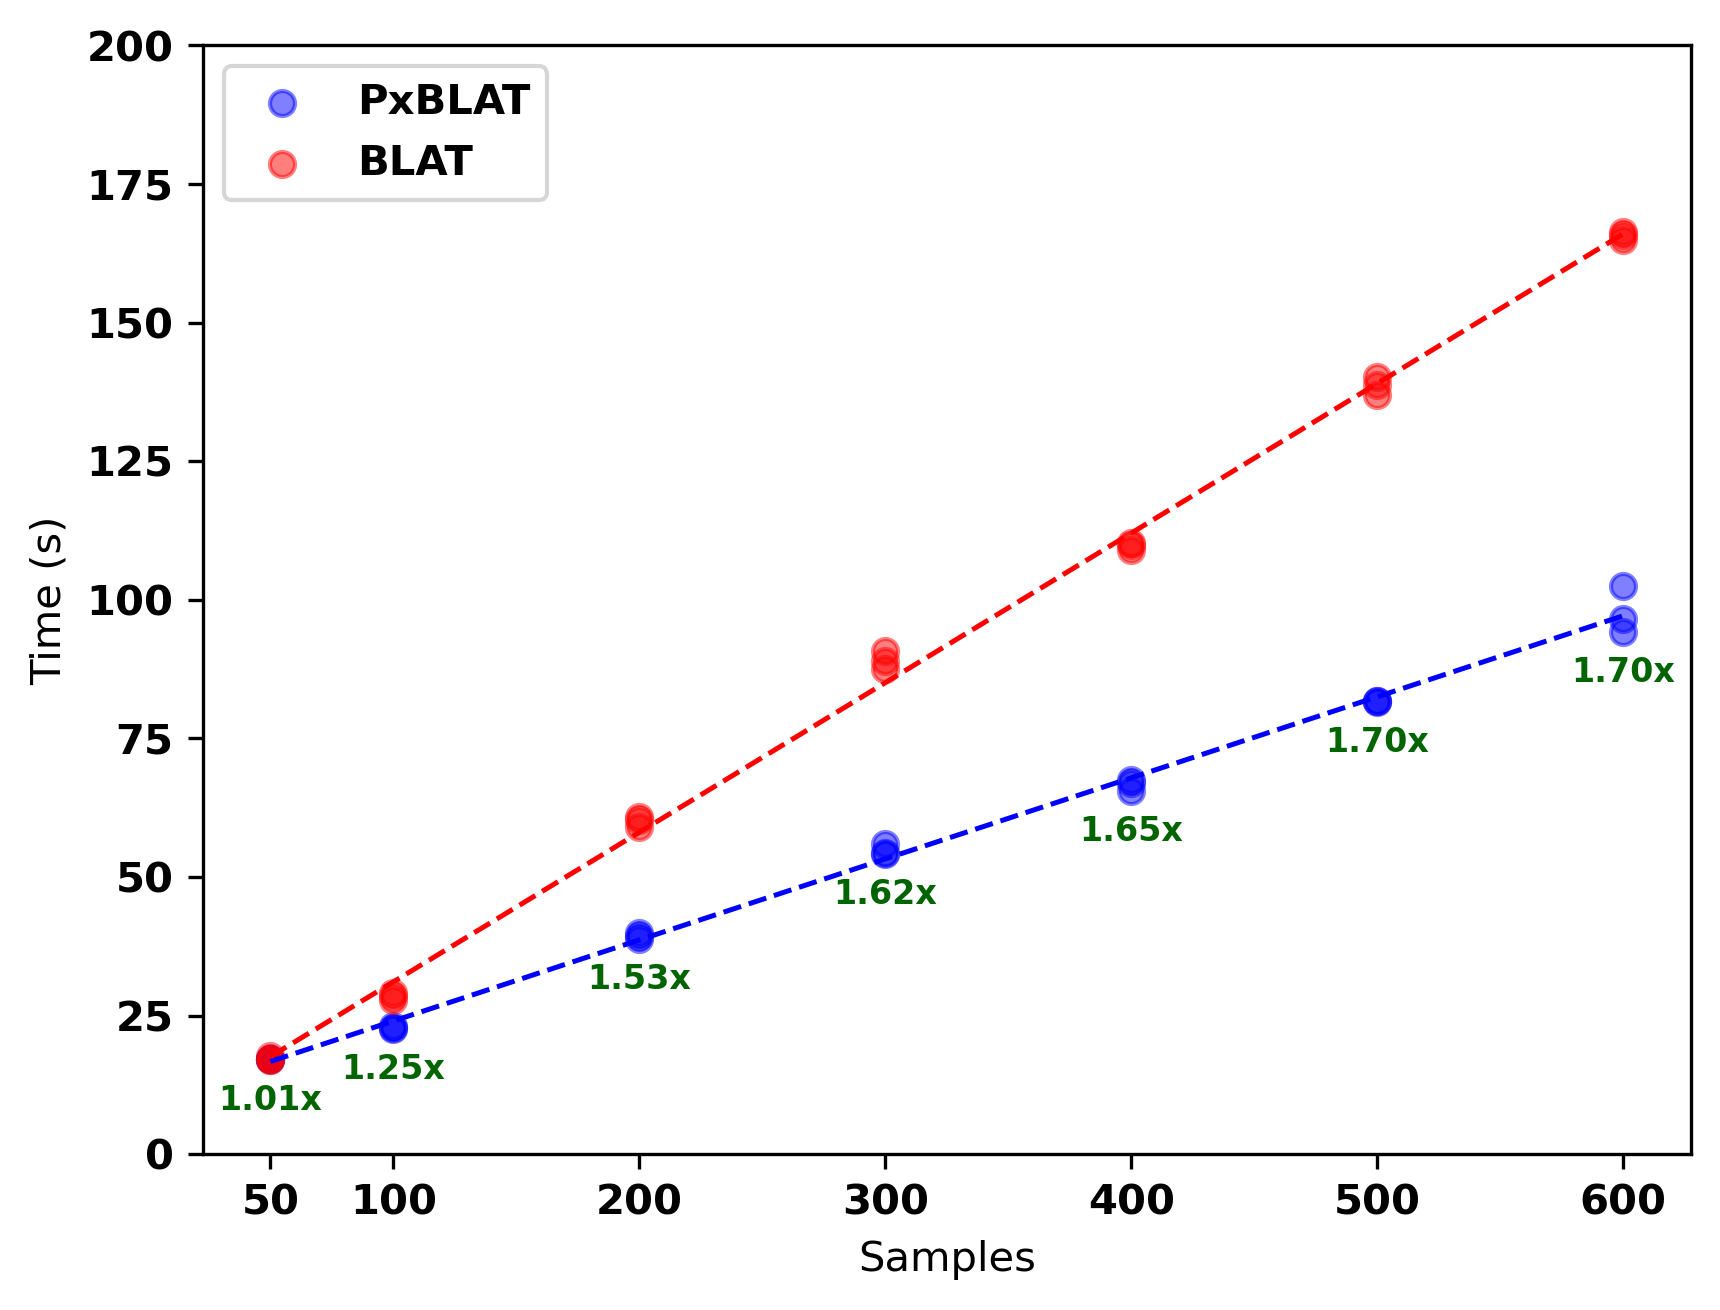
\includegraphics[width=\linewidth]{figures/performance}
	\caption{{\bf Performance comparison between \gls{blat} and \gls{pxblat}.} This figure quantifies the performance of \gls{blat} (indicated by red points) and \gls{pxblat} (indicated by blue points) across various data sets, with the \(x\) axis categorizing the number of samples in the sets and the \(y\) axis detailing the execution time in seconds.
		Each group encapsulates the results of three independent experiments.
		Trend lines, depicted in red for \gls{blat} and blue for \gls{pxblat}, illustrate the general performance pattern for each tool.
		Notably, the green text highlights the speedup achieved by PxBLAT, calculated as the ratio of the execution time (\(\mathrm{time}_\textsubscript{blat} / \mathrm{time}_\textsubscript{pxblat}\)), underscoring the efficiency gains of \gls{pxblat} relative to \gls{blat}.}
	\label{fig:performance}
\end{figure}

In summary, \gls{pxblat} demonstrates significant advantages in terms of execution time reduction.
These findings underscore its utility as a substantial improvement over the \gls{blat}, reinforcing its value within the bioinformatics toolkit.


%\begin{figure}[h]
%\centering
%
\includegraphics[width=0.9\textwidth]{fig.eps}
%\caption{This is a widefig. This is an example of long caption this is an example of long caption  this is an example of long caption this is an example of long caption}\label{fig1}
%\end{figure}
%
%In case of double column layout, the above format puts figure captions/images to single column width. To get spanned images, we need to provide \verb+\begin{figure*}+ \verb+...+ \verb+\end{figure*}+.
%
%For sample purpose, we have included the width of images in the optional argument of \verb+\includegraphics+ tag. Please ignore this.
%
%\section{Algorithms, Program codes and Listings}\label{sec7}
%
%Packages \verb+algorithm+, \verb+algorithmicx+ and \verb+algpseudocode+ are used for setting algorithms in \LaTeX\ using the format:

%%=============================================%%
%% For presentation purpose, we have included  %%
%% \bigskip command. Please ignore this.       %%
%%=============================================%%
%\bigskip
%\begin{verbatim}
%\begin{algorithm}
%\caption{<alg-caption>}\label{<alg-label>}
%\begin{algorithmic}[1]
%. . .
%\end{algorithmic}
%\end{algorithm}
%\end{verbatim}
%\bigskip
%%=============================================%%
%% For presentation purpose, we have included  %%
%% \bigskip command. Please ignore this.       %%
%%=============================================%%
%
%You may refer above listed package documentations for more details before setting \verb+algorithm+ environment. For program codes, the ``verbatim'' package is required and the command to be used is \verb+\begin{verbatim}+ \verb+...+ \verb+\end{verbatim}+.
%
%Similarly, for \verb+listings+, use the \verb+listings+ package. \verb+\begin{lstlisting}+ \verb+...+ \verb+\end{lstlisting}+ is used to set environments similar to \verb+verbatim+ environment. Refer to the \verb+lstlisting+ package documentation for more details.
%

%\section{Cross referencing}\label{sec8}
%
%Environments such as figure, table, equation and align can have a label
%declared via the \verb+\label{#label}+ command. For figures and table
%environments use the \verb+\label{}+ command inside or just
%below the \verb+\caption{}+ command. You can then use the
%\verb+\ref{#label}+ command to cross-reference them. As an example, consider
%the label declared for Figure~\ref{fig1} which is
%\verb+\label{fig1}+. To cross-reference it, use the command
%\verb+Figure \ref{fig1}+, for which it comes up as
%``Figure~\ref{fig1}''.
%
%To reference line numbers in an algorithm, consider the label declared for the line number 2 of Algorithm~\ref{algo1} is \verb+\label{algln2}+. To cross-reference it, use the command \verb+\ref{algln2}+ for which it comes up as line~\ref{algln2} of Algorithm~\ref{algo1}.
%
%\subsection{Details on reference citations}\label{subsec7}
%
%Standard \LaTeX\ permits only numerical citations. To support both numerical and author-year citations this template uses \verb+natbib+ \LaTeX\ package. For style guidance please refer to the template user manual.
%
%Here is an example for \verb+\cite{...}+: \cite{bib1}. Another example for \verb+\citep{...}+: \citep{bib2}. For author-year citation mode, \verb+\cite{...}+ prints Jones et al. (1990) and \verb+\citep{...}+ prints (Jones et al., 1990).
%
%All cited bib entries are printed at the end of this article: \cite{bib3}, \cite{bib4}, \cite{bib5}, \cite{bib6}, \cite{bib7}, \cite{bib8}, \cite{bib9}, \cite{bib10}, \cite{bib11}, \cite{bib12} and \cite{bib13}.


% \section{Discussion}\label{sec12}
% Discussions should be brief and focused. In some disciplines use of Discussion or `Conclusion' is interchangeable. It is not mandatory to use both. Some journals prefer a section `Results and Discussion' followed by a section `Conclusion'. Please refer to Journal-level guidance for any specific requirements.

\section{Conclusion}\label{sec:conclusion}
In conclusion, \gls{pxblat} is a robust, efficient, and user-friendly Python binding library designed to enhance the capabilities of \gls{blat}.
Its seamless integration with the Python ecosystem, coupled with its enhanced performance, underscores its potential to impact genomic data analysis workflows.
Overall, \gls{pxblat} provides a comprehensive set of features, including server management, data conversion utilities, and shell completion, to enhance the user experience.

\section{Availability and requirements}
\textbf{Project name}: \gls{pxblat}  \newline
\textbf{Project home page}: \url{https://github.com/ylab-hi/pxblat} \newline
\textbf{Operating system(s)}: Linux, Mac OS X  \newline
\textbf{Programming language}: C, C\texttt{++}, Python (version 3.9.0 or higher).  \newline
\textbf{Other requirements}: The source code and executables are freely available for academic, nonprofit and personal use. Commercial licensing information is available on the Kent Informatics website (\url{http://www.kentinformatics.com}).  \newline
\textbf{Any restrictions to use by non-academics}: license needed

\begin{appendices}

    \printglossary[type=\acronymtype, title=Abbreviations]
	
	% \section{Section title of first appendix}\label{secA1}
	% 
	% An appendix contains supplementary information that is not an essential part of the text itself but which may be helpful in providing a more comprehensive understanding of the research problem or it is information that is too cumbersome to be included in the body of the paper.
	
	%%=============================================%%
	%% For submissions to Nature Portfolio Journals %%
	%% please use the heading ``Extended Data''.   %%
	%%=============================================%%
	
	%%=============================================================%%
	%% Sample for another appendix section			       %%
	%%=============================================================%%
	
	%% \section{Example of another appendix section}\label{secA2}%
	%% Appendices may be used for helpful, supporting or essential material that would otherwise
	%% clutter, break up or be distracting to the text. Appendices can consist of sections, figures,
	%% tables and equations etc.
	
\end{appendices}

\backmatter
\bmhead{Supplementary information}

\paragraph*{S1 Table.}
\label{S1_Table}
{\bf Performance comparison between \gls{pxblat} and \gls{blat}.}
This table illustrates the performance of both \gls{pxblat} and \gls{blat} across data sets containing \num{50},  \num{100}, \num{200}, \num{300}, \num{400}, \num{500}, and \num{600} samples.
For each data set, three independent experiments are conducted to ensure robust performance evaluation.
The efficiency of \gls{pxblat} relative to \gls{blat} is quantified through the speedup metric, calculated as the ratio of the execution time (\(\mathrm{time}_\textsubscript{blat} / \mathrm{time}_\textsubscript{pxblat}\)).
This comparison highlights the computational advantages of \gls{pxblat} in terms of processing speed.

\begin{longtable}{SSSS}
	\toprule
	{Samples} & {PxBLAT (s)} & {BLAT (s)} & {Speedup} \\
	\midrule
	\endfirsthead
	\toprule
	{Samples} & {PxBLAT (s)} & {BLAT (s)} & {Speedup} \\
	\midrule
	\endhead
	\midrule
	\multicolumn{4}{r}{Continued on next page}        \\
	\midrule
	\endfoot
	\bottomrule
	\endlastfoot
	50        & 17.102400    & 17.034500  & 0.996030  \\
	50        & 17.092300    & 17.006900  & 0.995004  \\
	50        & 17.098200    & 17.722700  & 1.036524  \\
	100       & 22.749400    & 28.613600  & 1.257774  \\
	100       & 23.117700    & 29.097000  & 1.258646  \\
	100       & 22.534500    & 27.896400  & 1.237942  \\
	200       & 39.307500    & 59.027200  & 1.501678  \\
	200       & 38.859800    & 60.203200  & 1.549241  \\
	200       & 39.804700    & 60.873500  & 1.529304  \\
	300       & 55.893000    & 90.681000  & 1.622404  \\
	300       & 54.335900    & 88.877800  & 1.635710  \\
	300       & 54.154300    & 87.464200  & 1.615092  \\
	400       & 65.502000    & 110.204600 & 1.682462  \\
	400       & 67.017500    & 109.058900 & 1.627320  \\
	400       & 67.456100    & 109.789200 & 1.627565  \\
	500       & 81.555000    & 140.131900 & 1.718250  \\
	500       & 81.767500    & 138.657600 & 1.695754  \\
	500       & 81.730400    & 137.019200 & 1.676478  \\
	600       & 96.620400    & 165.867600 & 1.716693  \\
	600       & 102.548000   & 164.930200 & 1.608322  \\
	600       & 94.208100    & 166.379300 & 1.766083  \\
\end{longtable}

\paragraph*{S2 Table.}
\label{S2_Table}
{\bf \gls{hsp} comparison between \gls{pxblat} and \gls{blat}.}
This table, including \num{600} samples in total, presents a comparison of the \glspl{hsp} generated by \gls{blat} and \gls{pxblat} for each sample.
The column Sample lists the name of the sample, and the columns \gls{blat} and \gls{pxblat}, respectively denote the number of \glspl{hsp} generated by \gls{blat} and \gls{pxblat}.

\begin{longtable}{lSS}
	%    \caption{HSP Comparison between BLAT and PxBLAT} \label{tab:cmp} \\
	\toprule
	Sample                  & {BLAT} & {PxBLAT} \\
	\midrule
	\endfirsthead
	%	\caption[]{\gls{hsp} Comparison between BLAT and PxBLAT} \\
	\toprule
	Sample                  & {BLAT} & {PxBLAT} \\
	\midrule
	\endhead
	\midrule
	\multicolumn{3}{r}{Continued on next page}  \\
	\midrule
	\endfoot
	\bottomrule
	\endlastfoot
	chr20-11648866-11650925 & 130    & 130      \\
	chr20-29850079-29852595 & 1      & 1        \\
	chr20-7493878-7496145   & 26     & 26       \\
	chr20-30152074-30153892 & 3      & 3        \\
	chr20-1140095-1141788   & 22     & 22       \\
	chr20-17520690-17523557 & 14     & 14       \\
	chr20-41374266-41376291 & 12     & 12       \\
	chr20-63240773-63243242 & 64     & 64       \\
	chr20-59286740-59288091 & 13     & 13       \\
	chr20-8061734-8063508   & 10     & 10       \\
	chr20-34429296-34431248 & 41     & 41       \\
	chr20-27977914-27979241 & 22     & 22       \\
	chr20-11695455-11697457 & 20     & 20       \\
	chr20-41792348-41794797 & 131    & 131      \\
	chr20-25858004-25860351 & 37     & 37       \\
	chr20-31404034-31407027 & 25     & 25       \\
	chr20-15852904-15855300 & 65     & 65       \\
	chr20-29917054-29919227 & 18     & 18       \\
	chr20-45175162-45177033 & 2      & 2        \\
	chr20-43937342-43939507 & 58     & 58       \\
	chr20-17073859-17076499 & 48     & 48       \\
	chr20-19823346-19824950 & 32     & 32       \\
	chr20-28295597-28298301 & 23     & 23       \\
	chr20-15826504-15829187 & 26     & 26       \\
	chr20-54683378-54684991 & 47     & 47       \\
	chr20-55475241-55476377 & 18     & 18       \\
	chr20-57949934-57952283 & 74     & 74       \\
	chr20-14442978-14444604 & 35     & 35       \\
	chr20-51293808-51295630 & 38     & 38       \\
	chr20-49194155-49196823 & 165    & 165      \\
	chr20-34696351-34697788 & 43     & 43       \\
	chr20-16044321-16045712 & 48     & 48       \\
	chr20-45309757-45312553 & 39     & 39       \\
	chr20-21063232-21065145 & 26     & 26       \\
	chr20-434138-436331     & 174    & 174      \\
	chr20-62110486-62112604 & 167    & 167      \\
	chr20-15866914-15868171 & 15     & 15       \\
	chr20-62343940-62345043 & 69     & 69       \\
	chr20-37168356-37170160 & 34     & 34       \\
	chr20-15699683-15701260 & 15     & 15       \\
	chr20-44826183-44827333 & 152    & 152      \\
	chr20-41538435-41540074 & 43     & 43       \\
	chr20-56032843-56034378 & 18     & 18       \\
	chr20-36813618-36816516 & 21     & 21       \\
	chr20-18637848-18640751 & 68     & 68       \\
	chr20-56294086-56296598 & 27     & 27       \\
	chr20-19514094-19515343 & 2      & 2        \\
	chr20-33893321-33895564 & 126    & 126      \\
	chr20-22282380-22283429 & 4      & 4        \\
	chr20-39910629-39912740 & 84     & 84       \\
	chr20-40898874-40901542 & 27     & 27       \\
	chr20-7536153-7537696   & 15     & 15       \\
	chr20-4818626-4819858   & 60     & 60       \\
	chr20-64316707-64319236 & 24     & 24       \\
	chr20-2960440-2961833   & 119    & 119      \\
	chr20-2519249-2521676   & 46     & 46       \\
	chr20-11596878-11599706 & 68     & 68       \\
	chr20-30829536-30831739 & 16     & 16       \\
	chr20-45188854-45190558 & 3      & 3        \\
	chr20-47238745-47241145 & 14     & 14       \\
	chr20-10538965-10540232 & 83     & 83       \\
	chr20-11996320-11998343 & 87     & 87       \\
	chr20-23440919-23442976 & 47     & 47       \\
	chr20-22451495-22453568 & 4      & 4        \\
	chr20-39709672-39711911 & 23     & 23       \\
	chr20-29782708-29784088 & 8      & 8        \\
	chr20-7911434-7913178   & 9      & 9        \\
	chr20-1508550-1511129   & 193    & 193      \\
	chr20-41451172-41452837 & 6      & 6        \\
	chr20-4003988-4006545   & 29     & 29       \\
	chr20-10921197-10923149 & 5      & 5        \\
	chr20-36789016-36790500 & 186    & 186      \\
	chr20-9309222-9310479   & 157    & 157      \\
	chr20-52532795-52534564 & 9      & 9        \\
	chr20-42081563-42082983 & 4      & 4        \\
	chr20-12605319-12606971 & 2      & 2        \\
	chr20-29389010-29390598 & 149    & 149      \\
	chr20-8128132-8130266   & 170    & 170      \\
	chr20-11399422-11401237 & 12     & 12       \\
	chr20-33251227-33252414 & 2      & 2        \\
	chr20-3342256-3343645   & 92     & 92       \\
	chr20-38869283-38872088 & 60     & 60       \\
	chr20-7649152-7650444   & 60     & 60       \\
	chr20-13021673-13023769 & 58     & 58       \\
	chr20-3971117-3972667   & 32     & 32       \\
	chr20-26232703-26234929 & 61     & 61       \\
	chr20-23063517-23064745 & 7      & 7        \\
	chr20-39079691-39080763 & 26     & 26       \\
	chr20-23882126-23884119 & 92     & 92       \\
	chr20-3170215-3172728   & 44     & 44       \\
	chr20-49421601-49423499 & 35     & 35       \\
	chr20-55380779-55383730 & 204    & 204      \\
	chr20-45794728-45796900 & 164    & 164      \\
	chr20-15159613-15161221 & 9      & 9        \\
	chr20-62378279-62380174 & 184    & 184      \\
	chr20-6934771-6936584   & 116    & 116      \\
	chr20-59538484-59541329 & 8      & 8        \\
	chr20-43661982-43664714 & 26     & 26       \\
	chr20-36707842-36709247 & 85     & 85       \\
	chr20-33898085-33900435 & 65     & 65       \\
	chr20-18062688-18064265 & 46     & 46       \\
	chr20-29490152-29491491 & 23     & 23       \\
	chr20-30806959-30809757 & 0      & 0        \\
	chr20-11837593-11840377 & 40     & 40       \\
	chr20-28934655-28937276 & 1      & 1        \\
	chr20-7689471-7691553   & 18     & 18       \\
	chr20-1746811-1749803   & 9      & 9        \\
	chr20-1261408-1262588   & 16     & 16       \\
	chr20-5757029-5759548   & 29     & 29       \\
	chr20-5361957-5364278   & 107    & 107      \\
	chr20-37305589-37308001 & 21     & 21       \\
	chr20-53702835-53705300 & 148    & 148      \\
	chr20-7447290-7449191   & 16     & 16       \\
	chr20-36626015-36629010 & 150    & 150      \\
	chr20-48184357-48185678 & 2      & 2        \\
	chr20-4634043-4636057   & 9      & 9        \\
	chr20-21292878-21295830 & 179    & 179      \\
	chr20-52551672-52553086 & 7      & 7        \\
	chr20-55410142-55411547 & 55     & 55       \\
	chr20-15164296-15166007 & 21     & 21       \\
	chr20-60294852-60297789 & 197    & 197      \\
	chr20-47112993-47114241 & 38     & 38       \\
	chr20-33645643-33648541 & 62     & 62       \\
	chr20-57099663-57101555 & 91     & 91       \\
	chr20-32443012-32444528 & 1      & 1        \\
	chr20-54597242-54598325 & 31     & 31       \\
	chr20-28168758-28171348 & 20     & 20       \\
	chr20-14255274-14256294 & 211    & 211      \\
	chr20-22858139-22859797 & 8      & 8        \\
	chr20-42977157-42978222 & 11     & 11       \\
	chr20-3890553-3891667   & 46     & 46       \\
	chr20-10043505-10044872 & 33     & 33       \\
	chr20-47292153-47293840 & 50     & 50       \\
	chr20-30056354-30058719 & 0      & 0        \\
	chr20-23406092-23408775 & 15     & 15       \\
	chr20-44245002-44246392 & 36     & 36       \\
	chr20-30999482-31002350 & 1      & 1        \\
	chr20-11990150-11991239 & 3      & 3        \\
	chr20-3810992-3812466   & 197    & 197      \\
	chr20-26419101-26422061 & 0      & 0        \\
	chr20-22091287-22094021 & 119    & 119      \\
	chr20-47477509-47479589 & 59     & 59       \\
	chr20-13750647-13753070 & 44     & 44       \\
	chr20-61483678-61484972 & 2      & 2        \\
	chr20-57584630-57586794 & 13     & 13       \\
	chr20-17904728-17906925 & 34     & 34       \\
	chr20-28086098-28087474 & 19     & 19       \\
	chr20-21317295-21318548 & 51     & 51       \\
	chr20-42758324-42759488 & 193    & 193      \\
	chr20-23580801-23581810 & 23     & 23       \\
	chr20-58929386-58930631 & 22     & 22       \\
	chr20-6605062-6607136   & 79     & 79       \\
	chr20-32987534-32989963 & 169    & 169      \\
	chr20-22493043-22494805 & 22     & 22       \\
	chr20-54190709-54192035 & 24     & 24       \\
	chr20-48343887-48346044 & 2      & 2        \\
	chr20-10262876-10265171 & 189    & 189      \\
	chr20-35374558-35376267 & 67     & 67       \\
	chr20-39018648-39021540 & 83     & 83       \\
	chr20-37785924-37788264 & 202    & 202      \\
	chr20-64334961-64337760 & 0      & 0        \\
	chr20-12575681-12578297 & 14     & 14       \\
	chr20-23374273-23375283 & 1      & 1        \\
	chr20-14278920-14280350 & 40     & 40       \\
	chr20-42778102-42780755 & 9      & 9        \\
	chr20-52810557-52811573 & 83     & 83       \\
	chr20-52564945-52566606 & 22     & 22       \\
	chr20-10598821-10601808 & 32     & 32       \\
	chr20-1172826-1175431   & 87     & 87       \\
	chr20-3347653-3350627   & 44     & 44       \\
	chr20-64176870-64179763 & 43     & 43       \\
	chr20-42829128-42830258 & 100    & 100      \\
	chr20-40623645-40625957 & 187    & 187      \\
	chr20-27009229-27011878 & 24     & 24       \\
	chr20-14732847-14734481 & 95     & 95       \\
	chr20-12698635-12699679 & 2      & 2        \\
	chr20-13328590-13330614 & 13     & 13       \\
	chr20-22912395-22915205 & 12     & 12       \\
	chr20-35339375-35342113 & 48     & 48       \\
	chr20-19431509-19433187 & 28     & 28       \\
	chr20-28727730-28729750 & 16     & 16       \\
	chr20-39515806-39517118 & 2      & 2        \\
	chr20-21857448-21859310 & 209    & 209      \\
	chr20-44751640-44753567 & 19     & 19       \\
	chr20-47371415-47374127 & 45     & 45       \\
	chr20-24140371-24142959 & 6      & 6        \\
	chr20-54083025-54084528 & 41     & 41       \\
	chr20-51775800-51777458 & 46     & 46       \\
	chr20-59400225-59402632 & 30     & 30       \\
	chr20-57144627-57147621 & 47     & 47       \\
	chr20-17690928-17692128 & 6      & 6        \\
	chr20-31238605-31240139 & 4      & 4        \\
	chr20-29259215-29262074 & 4      & 4        \\
	chr20-39132690-39134466 & 34     & 34       \\
	chr20-44674003-44676622 & 31     & 31       \\
	chr20-34435089-34436815 & 13     & 13       \\
	chr20-11085268-11087065 & 27     & 27       \\
	chr20-42010931-42012642 & 10     & 10       \\
	chr20-7483012-7484115   & 1      & 1        \\
	chr20-39873233-39875635 & 207    & 207      \\
	chr20-32029134-32032031 & 93     & 93       \\
	chr20-38052616-38054138 & 32     & 32       \\
	chr20-2602976-2605324   & 19     & 19       \\
	chr20-42169915-42172757 & 15     & 15       \\
	chr20-62125729-62128471 & 19     & 19       \\
	chr20-2162753-2164165   & 5      & 5        \\
	chr20-34630972-34632436 & 113    & 113      \\
	chr20-6611620-6614440   & 152    & 152      \\
	chr20-19300360-19302642 & 6      & 6        \\
	chr20-25189802-25191365 & 154    & 154      \\
	chr20-15951964-15953450 & 26     & 26       \\
	chr20-47285001-47287102 & 52     & 52       \\
	chr20-22548369-22549974 & 9      & 9        \\
	chr20-24725480-24727693 & 52     & 52       \\
	chr20-55633941-55636718 & 5      & 5        \\
	chr20-30324027-30326285 & 30     & 30       \\
	chr20-34789703-34791591 & 27     & 27       \\
	chr20-22886111-22887126 & 5      & 5        \\
	chr20-52373722-52374925 & 52     & 52       \\
	chr20-62594615-62596270 & 61     & 61       \\
	chr20-23567798-23569994 & 5      & 5        \\
	chr20-52746782-52748970 & 26     & 26       \\
	chr20-63919107-63920159 & 20     & 20       \\
	chr20-37603411-37606081 & 21     & 21       \\
	chr20-45549091-45551404 & 167    & 167      \\
	chr20-24122821-24124880 & 2      & 2        \\
	chr20-39384970-39386746 & 47     & 47       \\
	chr20-56953750-56954962 & 11     & 11       \\
	chr20-27265832-27268665 & 27     & 27       \\
	chr20-989008-991475     & 96     & 96       \\
	chr20-13233506-13234845 & 9      & 9        \\
	chr20-30767954-30769153 & 0      & 0        \\
	chr20-54079315-54081921 & 56     & 56       \\
	chr20-22276591-22279281 & 202    & 202      \\
	chr20-32344273-32347087 & 26     & 26       \\
	chr20-14761627-14763228 & 15     & 15       \\
	chr20-24471803-24474607 & 7      & 7        \\
	chr20-22305788-22308754 & 43     & 43       \\
	chr20-63927315-63929626 & 54     & 54       \\
	chr20-33534721-33537439 & 158    & 158      \\
	chr20-53020990-53022920 & 33     & 33       \\
	chr20-44701412-44703325 & 34     & 34       \\
	chr20-63523339-63524524 & 190    & 190      \\
	chr20-39750571-39752199 & 50     & 50       \\
	chr20-47879542-47880820 & 162    & 162      \\
	chr20-12949055-12950079 & 1      & 1        \\
	chr20-37737796-37740734 & 26     & 26       \\
	chr20-17600492-17603407 & 68     & 68       \\
	chr20-40848143-40849212 & 2      & 2        \\
	chr20-33135173-33136880 & 131    & 131      \\
	chr20-39118192-39119260 & 4      & 4        \\
	chr20-27690465-27692366 & 23     & 23       \\
	chr20-37858061-37860321 & 49     & 49       \\
	chr20-12405605-12407882 & 6      & 6        \\
	chr20-57386121-57387852 & 70     & 70       \\
	chr20-34902889-34905611 & 39     & 39       \\
	chr20-52070637-52073331 & 35     & 35       \\
	chr20-40779660-40781751 & 47     & 47       \\
	chr20-31098450-31100717 & 3      & 3        \\
	chr20-29969458-29971235 & 18     & 18       \\
	chr20-13789470-13791842 & 152    & 152      \\
	chr20-26814485-26817257 & 22     & 22       \\
	chr20-40740691-40742983 & 29     & 29       \\
	chr20-49955693-49958425 & 183    & 183      \\
	chr20-37813305-37814584 & 9      & 9        \\
	chr20-18255943-18258048 & 64     & 64       \\
	chr20-63109432-63111043 & 34     & 34       \\
	chr20-14211039-14213272 & 9      & 9        \\
	chr20-17100441-17103140 & 9      & 9        \\
	chr20-2866996-2869328   & 38     & 38       \\
	chr20-53703835-53705398 & 158    & 158      \\
	chr20-51431118-51433743 & 56     & 56       \\
	chr20-6192786-6193790   & 196    & 196      \\
	chr20-10748356-10751019 & 35     & 35       \\
	chr20-33974548-33976407 & 44     & 44       \\
	chr20-32270385-32273111 & 20     & 20       \\
	chr20-36902282-36904506 & 28     & 28       \\
	chr20-198832-201190     & 40     & 40       \\
	chr20-7927314-7928574   & 27     & 27       \\
	chr20-17899461-17900502 & 58     & 58       \\
	chr20-11120841-11122366 & 23     & 23       \\
	chr20-59407661-59409193 & 27     & 27       \\
	chr20-35649824-35652625 & 5      & 5        \\
	chr20-30688628-30690580 & 48     & 48       \\
	chr20-49466264-49467309 & 5      & 5        \\
	chr20-63692672-63694078 & 2      & 2        \\
	chr20-12570747-12573421 & 5      & 5        \\
	chr20-8512304-8514491   & 20     & 20       \\
	chr20-24204303-24205314 & 2      & 2        \\
	chr20-11639430-11641175 & 20     & 20       \\
	chr20-26938330-26940788 & 24     & 24       \\
	chr20-17587799-17589501 & 209    & 209      \\
	chr20-26384682-26386149 & 23     & 23       \\
	chr20-46308421-46310414 & 41     & 41       \\
	chr20-30072951-30074554 & 0      & 0        \\
	chr20-44079162-44081096 & 23     & 23       \\
	chr20-21475551-21476686 & 50     & 50       \\
	chr20-13972488-13974627 & 44     & 44       \\
	chr20-45697903-45699479 & 88     & 88       \\
	chr20-24838480-24839925 & 11     & 11       \\
	chr20-7742386-7745111   & 4      & 4        \\
	chr20-56522851-56524815 & 12     & 12       \\
	chr20-22497057-22499773 & 16     & 16       \\
	chr20-51998729-52000293 & 22     & 22       \\
	chr20-38767581-38768689 & 5      & 5        \\
	chr20-19863311-19865822 & 56     & 56       \\
	chr20-9295230-9297764   & 226    & 226      \\
	chr20-15012779-15015584 & 8      & 8        \\
	chr20-5041846-5044587   & 56     & 56       \\
	chr20-580210-582022     & 35     & 35       \\
	chr20-15328579-15331324 & 42     & 42       \\
	chr20-49481967-49483214 & 17     & 17       \\
	chr20-5260817-5262044   & 5      & 5        \\
	chr20-23340929-23343084 & 102    & 102      \\
	chr20-2269716-2270774   & 189    & 189      \\
	chr20-46399947-46401667 & 31     & 31       \\
	chr20-10815100-10817410 & 32     & 32       \\
	chr20-45864818-45866440 & 53     & 53       \\
	chr20-45489949-45492069 & 35     & 35       \\
	chr20-21302718-21304312 & 1      & 1        \\
	chr20-9931834-9933992   & 5      & 5        \\
	chr20-56295194-56296721 & 5      & 5        \\
	chr20-38225781-38227971 & 18     & 18       \\
	chr20-18585659-18587381 & 35     & 35       \\
	chr20-16940912-16942721 & 39     & 39       \\
	chr20-3758200-3759977   & 4      & 4        \\
	chr20-11807056-11808124 & 3      & 3        \\
	chr20-127575-129488     & 93     & 93       \\
	chr20-40755444-40756701 & 5      & 5        \\
	chr20-21011682-21013735 & 2      & 2        \\
	chr20-10119043-10120171 & 59     & 59       \\
	chr20-1313128-1315640   & 18     & 18       \\
	chr20-11712977-11715178 & 142    & 142      \\
	chr20-34597997-34600726 & 28     & 28       \\
	chr20-53048517-53050101 & 29     & 29       \\
	chr20-15161566-15163488 & 8      & 8        \\
	chr20-15137364-15139959 & 203    & 203      \\
	chr20-60342420-60345056 & 94     & 94       \\
	chr20-55169861-55170982 & 156    & 156      \\
	chr20-24314101-24316265 & 27     & 27       \\
	chr20-53183314-53186148 & 16     & 16       \\
	chr20-43887385-43889661 & 75     & 75       \\
	chr20-59470391-59471545 & 1      & 1        \\
	chr20-53159093-53161302 & 35     & 35       \\
	chr20-5895129-5896312   & 26     & 26       \\
	chr20-25292499-25293803 & 3      & 3        \\
	chr20-34161145-34162369 & 41     & 41       \\
	chr20-45868564-45870103 & 74     & 74       \\
	chr20-4887453-4889888   & 3      & 3        \\
	chr20-39559840-39561722 & 9      & 9        \\
	chr20-33221436-33223116 & 56     & 56       \\
	chr20-755464-758088     & 35     & 35       \\
	chr20-1111176-1112831   & 46     & 46       \\
	chr20-2802607-2803838   & 36     & 36       \\
	chr20-38997152-38999498 & 22     & 22       \\
	chr20-5049946-5052675   & 35     & 35       \\
	chr20-48767423-48769196 & 48     & 48       \\
	chr20-2659893-2661452   & 56     & 56       \\
	chr20-49121260-49124086 & 21     & 21       \\
	chr20-54247731-54250009 & 75     & 75       \\
	chr20-8334685-8337480   & 34     & 34       \\
	chr20-26427340-26428991 & 0      & 0        \\
	chr20-1762478-1764560   & 46     & 46       \\
	chr20-53286968-53289954 & 23     & 23       \\
	chr20-23613637-23615158 & 53     & 53       \\
	chr20-7135001-7136753   & 88     & 88       \\
	chr20-59872605-59875175 & 5      & 5        \\
	chr20-33944307-33946354 & 27     & 27       \\
	chr20-29344297-29347205 & 8      & 8        \\
	chr20-28334593-28336360 & 22     & 22       \\
	chr20-49230825-49232042 & 66     & 66       \\
	chr20-48044237-48045631 & 3      & 3        \\
	chr20-26227485-26229228 & 5      & 5        \\
	chr20-26487906-26489572 & 25     & 25       \\
	chr20-11596974-11599728 & 65     & 65       \\
	chr20-45661385-45663135 & 194    & 194      \\
	chr20-23562380-23564047 & 2      & 2        \\
	chr20-5735736-5738602   & 12     & 12       \\
	chr20-31727237-31729024 & 39     & 39       \\
	chr20-36152090-36154966 & 151    & 151      \\
	chr20-1018906-1020553   & 11     & 11       \\
	chr20-9821106-9823172   & 75     & 75       \\
	chr20-52034533-52037144 & 85     & 85       \\
	chr20-15008181-15010280 & 66     & 66       \\
	chr20-41851737-41853531 & 6      & 6        \\
	chr20-29408974-29411107 & 20     & 20       \\
	chr20-10955881-10957008 & 1      & 1        \\
	chr20-8970270-8971572   & 18     & 18       \\
	chr20-2350436-2352589   & 200    & 200      \\
	chr20-35494115-35496325 & 37     & 37       \\
	chr20-16994461-16996880 & 203    & 203      \\
	chr20-1121638-1123536   & 20     & 20       \\
	chr20-10539946-10542788 & 76     & 76       \\
	chr20-31981394-31984035 & 24     & 24       \\
	chr20-31059406-31062015 & 9      & 9        \\
	chr20-23005241-23006490 & 85     & 85       \\
	chr20-27678668-27680740 & 22     & 22       \\
	chr20-23089029-23090440 & 1      & 1        \\
	chr20-18766639-18768846 & 74     & 74       \\
	chr20-35270491-35271927 & 24     & 24       \\
	chr20-32671767-32673927 & 46     & 46       \\
	chr20-5469364-5470405   & 1      & 1        \\
	chr20-44586665-44588074 & 3      & 3        \\
	chr20-19751371-19752469 & 50     & 50       \\
	chr20-11475039-11477338 & 4      & 4        \\
	chr20-52930875-52933353 & 52     & 52       \\
	chr20-23941121-23942933 & 189    & 189      \\
	chr20-10612667-10615654 & 16     & 16       \\
	chr20-39220431-39222072 & 6      & 6        \\
	chr20-24056618-24059198 & 190    & 190      \\
	chr20-63753892-63756615 & 196    & 196      \\
	chr20-64298054-64301011 & 16     & 16       \\
	chr20-43632072-43634462 & 46     & 46       \\
	chr20-29402266-29403661 & 49     & 49       \\
	chr20-34611441-34612505 & 39     & 39       \\
	chr20-16219627-16222599 & 19     & 19       \\
	chr20-47623287-47624373 & 18     & 18       \\
	chr20-37572653-37574987 & 20     & 20       \\
	chr20-57328038-57329145 & 159    & 159      \\
	chr20-54255861-54257299 & 11     & 11       \\
	chr20-17523656-17525455 & 3      & 3        \\
	chr20-3054439-3055812   & 26     & 26       \\
	chr20-51095602-51096740 & 8      & 8        \\
	chr20-26295259-26296843 & 6      & 6        \\
	chr20-16956946-16959866 & 4      & 4        \\
	chr20-59871467-59873730 & 18     & 18       \\
	chr20-12972124-12973571 & 9      & 9        \\
	chr20-64187505-64190371 & 7      & 7        \\
	chr20-20036801-20038441 & 54     & 54       \\
	chr20-52361579-52363650 & 49     & 49       \\
	chr20-48763637-48765211 & 21     & 21       \\
	chr20-29272745-29274078 & 3      & 3        \\
	chr20-6596603-6597647   & 1      & 1        \\
	chr20-25092945-25094053 & 38     & 38       \\
	chr20-23976043-23978934 & 34     & 34       \\
	chr20-33528290-33530524 & 183    & 183      \\
	chr20-45968564-45971166 & 41     & 41       \\
	chr20-29195839-29197450 & 17     & 17       \\
	chr20-12991634-12993772 & 18     & 18       \\
	chr20-7287285-7289523   & 45     & 45       \\
	chr20-12780972-12782351 & 20     & 20       \\
	chr20-17273569-17275885 & 46     & 46       \\
	chr20-53404329-53405379 & 8      & 8        \\
	chr20-32199416-32201827 & 159    & 159      \\
	chr20-56899277-56900938 & 64     & 64       \\
	chr20-21026086-21027263 & 198    & 198      \\
	chr20-29495766-29497356 & 5      & 5        \\
	chr20-46509725-46510768 & 176    & 176      \\
	chr20-44370323-44372070 & 36     & 36       \\
	chr20-34807421-34810326 & 128    & 128      \\
	chr20-29310629-29312542 & 80     & 80       \\
	chr20-1861413-1862970   & 10     & 10       \\
	chr20-13425759-13427299 & 2      & 2        \\
	chr20-40797946-40799834 & 14     & 14       \\
	chr20-9134988-9136715   & 38     & 38       \\
	chr20-6129194-6130506   & 20     & 20       \\
	chr20-32328850-32331341 & 40     & 40       \\
	chr20-37816931-37818838 & 30     & 30       \\
	chr20-43643216-43645801 & 82     & 82       \\
	chr20-57951819-57954389 & 39     & 39       \\
	chr20-38495333-38497995 & 69     & 69       \\
	chr20-23579562-23580734 & 13     & 13       \\
	chr20-32476687-32477738 & 89     & 89       \\
	chr20-46657968-46660258 & 17     & 17       \\
	chr20-44029371-44030373 & 1      & 1        \\
	chr20-19040746-19042992 & 24     & 24       \\
	chr20-41547378-41548428 & 5      & 5        \\
	chr20-31338848-31340507 & 33     & 33       \\
	chr20-50733531-50736468 & 30     & 30       \\
	chr20-23264110-23266210 & 46     & 46       \\
	chr20-59975068-59976189 & 25     & 25       \\
	chr20-40116512-40117628 & 2      & 2        \\
	chr20-34348380-34351135 & 191    & 191      \\
	chr20-53857114-53859581 & 90     & 90       \\
	chr20-24510328-24512009 & 40     & 40       \\
	chr20-2400648-2401902   & 51     & 51       \\
	chr20-41951417-41953958 & 8      & 8        \\
	chr20-10519505-10521311 & 173    & 173      \\
	chr20-38229341-38232239 & 39     & 39       \\
	chr20-1961461-1962512   & 4      & 4        \\
	chr20-4493702-4496293   & 164    & 164      \\
	chr20-39058190-39059640 & 65     & 65       \\
	chr20-11840010-11842763 & 159    & 159      \\
	chr20-51385931-51387697 & 2      & 2        \\
	chr20-32743241-32746228 & 61     & 61       \\
	chr20-36043748-36044868 & 4      & 4        \\
	chr20-47940674-47941937 & 27     & 27       \\
	chr20-22906294-22908788 & 8      & 8        \\
	chr20-46563742-46565560 & 42     & 42       \\
	chr20-34970963-34972526 & 22     & 22       \\
	chr20-46825075-46827145 & 11     & 11       \\
	chr20-6428315-6430827   & 188    & 188      \\
	chr20-42217777-42219934 & 16     & 16       \\
	chr20-19913134-19914585 & 34     & 34       \\
	chr20-37718004-37720318 & 152    & 152      \\
	chr20-51873445-51875614 & 85     & 85       \\
	chr20-21185966-21187683 & 41     & 41       \\
	chr20-36715891-36717659 & 71     & 71       \\
	chr20-25706788-25709614 & 123    & 123      \\
	chr20-50918346-50919658 & 55     & 55       \\
	chr20-19216584-19217715 & 110    & 110      \\
	chr20-60913180-60914343 & 27     & 27       \\
	chr20-40445916-40447302 & 2      & 2        \\
	chr20-39471792-39473038 & 200    & 200      \\
	chr20-36763453-36764650 & 82     & 82       \\
	chr20-58906803-58909272 & 170    & 170      \\
	chr20-24358042-24359864 & 9      & 9        \\
	chr20-5054910-5055935   & 113    & 113      \\
	chr20-39718409-39719767 & 60     & 60       \\
	chr20-48995874-48997427 & 47     & 47       \\
	chr20-11060084-11062288 & 61     & 61       \\
	chr20-3041121-3043902   & 46     & 46       \\
	chr20-11729530-11731335 & 4      & 4        \\
	chr20-6876021-6878545   & 44     & 44       \\
	chr20-60459034-60461357 & 22     & 22       \\
	chr20-50558110-50560711 & 68     & 68       \\
	chr20-1551191-1553332   & 2      & 2        \\
	chr20-23189149-23191563 & 50     & 50       \\
	chr20-46682255-46683957 & 5      & 5        \\
	chr20-46693319-46694364 & 56     & 56       \\
	chr20-50170226-50172189 & 11     & 11       \\
	chr20-63698924-63701762 & 5      & 5        \\
	chr20-62756096-62757580 & 69     & 69       \\
	chr20-55371351-55373202 & 30     & 30       \\
	chr20-61650045-61652414 & 3      & 3        \\
	chr20-33091750-33093858 & 24     & 24       \\
	chr20-61216684-61218692 & 7      & 7        \\
	chr20-47978091-47980293 & 85     & 85       \\
	chr20-16870384-16872626 & 14     & 14       \\
	chr20-55265469-55267149 & 6      & 6        \\
	chr20-42713744-42715938 & 38     & 38       \\
	chr20-20608914-20611491 & 36     & 36       \\
	chr20-59966328-59967826 & 57     & 57       \\
	chr20-29829808-29831310 & 8      & 8        \\
	chr20-55321262-55323731 & 34     & 34       \\
	chr20-38905281-38906801 & 57     & 57       \\
	chr20-5081835-5084428   & 35     & 35       \\
	chr20-12399681-12402397 & 19     & 19       \\
	chr20-15787670-15789236 & 10     & 10       \\
	chr20-61849267-61851471 & 112    & 112      \\
	chr20-42224821-42226456 & 8      & 8        \\
	chr20-2200973-2202184   & 2      & 2        \\
	chr20-44016368-44018208 & 138    & 138      \\
	chr20-42732744-42735046 & 2      & 2        \\
	chr20-8901543-8903090   & 37     & 37       \\
	chr20-33361770-33363718 & 16     & 16       \\
	chr20-60319529-60322435 & 17     & 17       \\
	chr20-9417083-9419320   & 19     & 19       \\
	chr20-47368389-47371245 & 181    & 181      \\
	chr20-49829087-49831301 & 97     & 97       \\
	chr20-45577205-45579659 & 30     & 30       \\
	chr20-9885847-9887724   & 4      & 4        \\
	chr20-34086336-34087450 & 25     & 25       \\
	chr20-12690873-12693547 & 25     & 25       \\
	chr20-61265483-61267506 & 31     & 31       \\
	chr20-60767473-60770234 & 21     & 21       \\
	chr20-37096290-37097735 & 46     & 46       \\
	chr20-19806699-19808018 & 39     & 39       \\
	chr20-5383554-5385658   & 41     & 41       \\
	chr20-46475786-46476831 & 62     & 62       \\
	chr20-35346166-35347602 & 30     & 30       \\
	chr20-39431060-39432816 & 28     & 28       \\
	chr20-50643697-50644883 & 205    & 205      \\
	chr20-22403148-22404794 & 15     & 15       \\
	chr20-26331430-26334030 & 3      & 3        \\
	chr20-14375436-14376511 & 196    & 196      \\
	chr20-32839818-32840903 & 124    & 124      \\
	chr20-20727967-20730763 & 59     & 59       \\
	chr20-25447522-25449068 & 21     & 21       \\
	chr20-52094840-52096680 & 143    & 143      \\
	chr20-21563954-21565882 & 146    & 146      \\
	chr20-5436550-5437659   & 70     & 70       \\
	chr20-63482588-63484649 & 191    & 191      \\
	chr20-19772825-19774949 & 43     & 43       \\
	chr20-38393781-38395769 & 19     & 19       \\
	chr20-34751103-34754059 & 175    & 175      \\
	chr20-26987677-26990651 & 24     & 24       \\
	chr20-8530344-8531955   & 41     & 41       \\
	chr20-2975561-2977607   & 0      & 0        \\
	chr20-56181870-56183051 & 0      & 0        \\
	chr20-35814820-35817469 & 0      & 0        \\
	chr20-13176813-13178454 & 0      & 0        \\
	chr20-45598592-45599763 & 0      & 0        \\
	chr20-23037040-23038387 & 0      & 0        \\
	chr20-17554036-17556666 & 0      & 0        \\
	chr20-59732533-59734709 & 0      & 0        \\
	chr20-43253525-43256343 & 0      & 0        \\
	chr20-5541509-5543311   & 0      & 0        \\
	chr20-48761025-48762893 & 0      & 0        \\
	chr20-34464744-34466642 & 0      & 0        \\
	chr20-42866256-42868185 & 0      & 0        \\
	chr20-50226595-50228543 & 0      & 0        \\
	chr20-43868259-43870002 & 0      & 0        \\
	chr20-61460131-61461808 & 0      & 0        \\
	chr20-18061681-18062812 & 0      & 0        \\
	chr20-33365416-33368097 & 0      & 0        \\
	chr20-15504260-15505833 & 0      & 0        \\
	chr20-14468799-14471029 & 0      & 0        \\
	chr20-3363803-3366253   & 0      & 0        \\
	chr20-15709653-15710930 & 0      & 0        \\
\end{longtable}




% \section*{Declarations}

% Some journals require declarations to be submitted in a standardised format.
% Please check the Instructions for Authors of the journal to which you are submitting to see if you need to complete this section.
% If yes, your manuscript must contain the following sections under the heading `Declarations':
\bmhead{Availability of data and materials}
The \gls{pxblat}, along with the source code, is publicly available in the GitHub repository at \url{https://github.com/ylab-hi/pxblat}.
The documentation is available at ReadtheDocs \url{https://pxblat.readthedocs.io/en/latest/}.
The script for benchmarking is available at \emph{tests/test\_result.py} in the repository.
The testing dataset is available at the GitHub repository {\url{https://github.com/ylab-hi/pxblat}.
The path of the testing dataset is \emph{benchmark/fas}.

\bmhead{Competing interests}
No competing interest is declared.

\bmhead{Funding}
This work was supported by the National Institute of General Medical
Sciences [R35GM142441].

\bmhead{Authors' contributions}
Y.L. and R.Y. conceptualized the project. Y.L. implemented the software and conducted the benchmarking. R.Y. supervised the project. Both authors wrote the manuscript. All authors read and approved the final manuscript.

\bmhead{Acknowledgements}

Special thanks to the team who maintain the \gls{ucsc} codebase and users from the bioinformatics community whose valuable feedback and suggestions were pivotal in refining \gls{pxblat}'s design and functionality.


% \begin{itemize}
% 	\item Funding
% 	\item Conflict of interest/Competing interests (check journal-specific guidelines for which heading to use)
% 	\item Ethics approval and consent to participate
% 	\item Consent for publication
% 	\item Data availability
% 	\item Materials availability
% 	\item Code availability
% 	\item Author contribution
% \end{itemize}

% \noindent
% If any of the sections are not relevant to your manuscript, please include the heading and write `Not applicable' for that section.

%%===================================================%%
%% For presentation purpose, we have included        %%
%% \bigskip command. Please ignore this.             %%
%%===================================================%%
% \bigskip
% \begin{flushleft}%
% 	Editorial Policies for:
%
% 	\bigskip\noindent
% 	Springer journals and proceedings: \url{https://www.springer.com/gp/editorial-policies}
%
% 	\bigskip\noindent
% 	Nature Portfolio journals: \url{https://www.nature.com/nature-research/editorial-policies}
%
% 	\bigskip\noindent
% 	\textit{Scientific Reports}: \url{https://www.nature.com/srep/journal-policies/editorial-policies}
%
% 	\bigskip\noindent
% 	BMC journals: \url{https://www.biomedcentral.com/getpublished/editorial-policies}
% \end{flushleft}

%%===========================================================================================%%
%% If you are submitting to one of the Nature Portfolio journals, using the eJP submission   %%
%% system, please include the references within the manuscript file itself. You may do this  %%
%% by copying the reference list from your .bbl file, paste it into the main manuscript .tex %%
%% file, and delete the associated \verb+\bibliography+ commands.                            %%
%%===========================================================================================%%

\bibliography{ref}% common bib file
%% if required, the content of .bbl file can be included here once bbl is generated
%%\input sn-article.bbl


\end{document}
